\documentclass[10pt,twocolumn,letterpaper]{article}

\usepackage{cvpr}
\usepackage{times}
\usepackage{epsfig}
\usepackage{graphicx}
\usepackage{amsmath}
\usepackage{amssymb}
\usepackage[euler]{textgreek}
\usepackage{multirow}
\usepackage{graphicx}
\usepackage{booktabs}

% Include other packages here, before hyperref.

% If you comment hyperref and then uncomment it, you should delete
% egpaper.aux before re-running latex.  (Or just hit 'q' on the first latex
% run, let it finish, and you should be clear).
\usepackage[pagebackref=true,breaklinks=true,letterpaper=true,colorlinks,bookmarks=false]{hyperref}

\cvprfinalcopy % *** Uncomment this line for the final submission

\def\cvprPaperID{****} % *** Enter the CVPR Paper ID here
\def\httilde{\mbox{\tt\raisebox{-.5ex}{\symbol{126}}}}
% Pages are numbered in submission mode, and unnumbered in camera-ready
\ifcvprfinal\pagestyle{empty}\fi
\begin{document}

%%%%%%%%% TITLE
\title{Severstal steel defect segmentation \\ IACV 2019-2020 Project} 

\author{Andrea Bionda\\
Politecnico di Milano\\
{\tt\small andrea.bionda@mail.polimi.it}}

\maketitle
%\thispagestyle{empty}

%%%%%%%%% ABSTRACT
\begin{abstract}
   It has been observed that the future of metallurgy requires the development of even more technological tools to face contemporary economic, ecological, and social challenges.
   The purpose of this paper is to provide a deep learning approach for the segmentation and classification of defects on steel sheets.\\
   The proposed solution is built focusing on two expected results: a precise defect segmentation and labelling, and an accurate classification between defective and non-defective images, in order to reduce false positives, and so waste of money and resources.\\
   I will try to solve the above problem, using a combination of two famous deep learning approaches, named image classification and semantic segmentation, respectively.
   The evaluation metrics is the so called Dice coefficient, which is not only an accuracy index, but it also penalizes the false positives found by the method, more similar to precision.
\end{abstract}

%%%%%%%%% INTRODUCTION
%------------------------------------------------------------------------
\graphicspath{ {./Resources/} }
\section{Introduction}
   In order to increase efficiency in production, Severstal collected gigabytes of data looking for a deep learning approach that helps them in the problem of recognizing and classifying automatically surface defects on steel sheets. The semantic segmentation aims to provide a label for each pixel in the image, that in relation to this problem means to assign one of the four defective classes or the non-defective ones to each pixel.\\
   The main contribution of this paper is to present a method which results to be a good tradeoff between accuracy on defect segmentation and precision in defective-image identification. The proposed solution takes in input images of steel sheets that come from high-frequency cameras and outputs the same-size segmented images, which contain the area of the identified defect(s) (if any) and the corresponding type. \\
   The first explored approach is to use a single Fully Convolutional Neural Network that performs semantic segmentation over the four defects; in particular, I have used the U-Net architecture. This method gives a Dice coefficient of 0.6 in the test set.
   In order to improve precision, and so to reduce false positives, the second approach is a pipeline of two different techniques: in the first stage, there is a Binary Classifier that is trained to filter out defect-free images; in the second stage, it is placed the segmentation model presented in the first method, that will segment only images that are labelled defective by the Classifier. This second approach gives a Dice coefficient of 0.73 in the test set.\\ 
   The rationale behind the pipeline is not to let the U-Net worry about the possibility of identifying false defects, that usually have a very similar pattern compared to real defects (Figure \ref{fig:result2}), in order not to reduce its segmentation ability too much; then the idea follows with the training of a classification model with the purpose to find and filter out non-defective images.\\
   The images come from real camera shots of steel sheets and can present 4 types of defects, classified in: Pitting (Figure \ref{fig:defect1}), Inclusion (Figure \ref{fig:defect2}), Scratches (Figure \ref{fig:defect3}) and Corrosion (Figure \ref{fig:defect4}).
   
   \begin{figure}[h]
      \centering
      \caption{Pitting} \label{fig:defect1}
      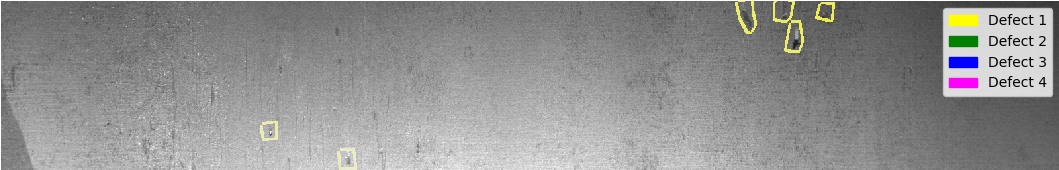
\includegraphics[scale=0.3]{Img_Defect1}
      \caption{Inclusion} \label{fig:defect2}
      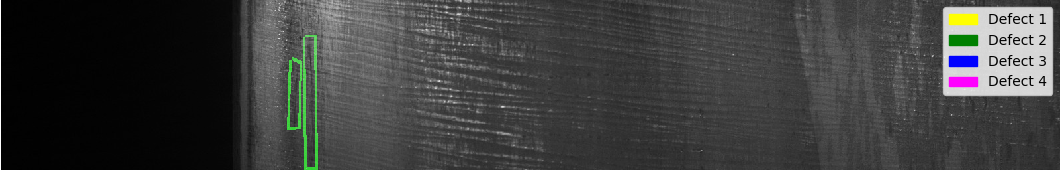
\includegraphics[scale=0.3]{Img_Defect2}
      \caption{Scratches} \label{fig:defect3}
      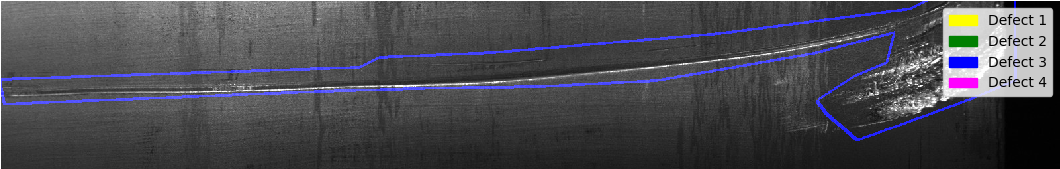
\includegraphics[scale=0.3]{Img_Defect3}
      \caption{Corrosion} \label{fig:defect4}
      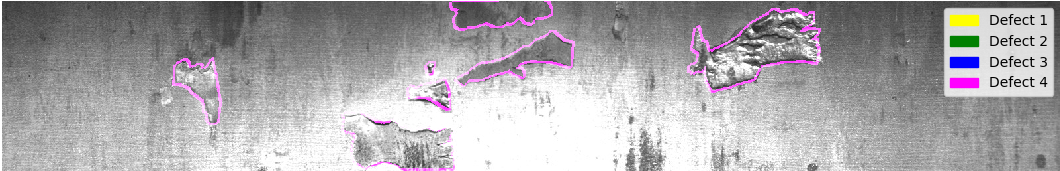
\includegraphics[scale=0.3]{Img_Defect4}
   \end{figure}


%%%%%%%%% RELATED WORK
%------------------------------------------------------------------------
\section{Related work}
   Since the output of the problem is a pixel-wise label for the input image, it is essentially a semantic segmentation task. In our case, it is also used a binary classifier to refine the results.
   \subsection{Residual Networks} 
      This family of Convolutional Neural Networks is built to face the degradation problem of very deep networks. The related paper proposes that such degradation is not caused by overfitting, but instead it is due to the well-known vanishing gradient issue. The main idea is to add an identity shortcut connection between blocks (group of convolutional layers), in such a way that each one learns features from both the previous block and the input value \cite{resnet}.
      In this paper, I will refer to ResNet34 and ResNet50, two models of the same family, but with different number of layers.
   \subsection{EfficientNet}
      The idea behind this family of Convolutional Neural Networks is to scale a baseline model, called EfficientNet-B0, in width, depth, and resolution by a costant ratio, in order to obtain higher accuracy. This process allows to keep the number of parameters lower than the one in same accuracy-level models \cite{efficientnet}. In the proposed solution, I will refer to EfficientNet-B3, a good tradeoff between accuracy level and network size.
   \subsection{U-Net}
      The baseline architecture used in the segmentation phase is the so called U-Net, that is composed of two concatenated parts: the contracting path (or down-sampling network or encoder network) works as a classical Fully Convolutional Neural Network (FCNN) to extract meaningful features from the image, while the expansive path (or up-sampling network or decoder network) builds a high resolution output, starting from the feature extracted during the first phase. The biggest contribution taken by this architecture is that each up-sampling layer is enriched with feature information extracted in the corresponding downsampling layer, in order to achieve higher semantic levels \cite{Unet}. 



%%%%%%%%% PROPOSED APPROACH
%------------------------------------------------------------------------
\section{Proposed approach}
   The first and straightforward solution that I have applied to the problem is to build a U-Net architecture for semantic segmentation in such a way that it outputs same-size images with 4 channels, one for each defect class (Figure \ref{fig:firstApproach}).  
   Each channel (layer) of the output represents the heatmap (image where, for each pixel, a probability that it belongs to a defect in the original image is assigned) of the corresponding defect class. 

   \begin{figure}[h]
      \centering
      \caption{First approach: segmentation inference only} \label{fig:firstApproach}
      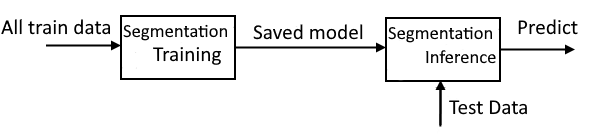
\includegraphics[scale=0.55]{Img_FirstApproach}
   \end{figure}

   This method has a very good capibility in defect recognition, but at the same time it hardly distinguishes real defects from the false ones, due to their similar pattern (an example on Figure \ref{fig:result1} and \ref{fig:result2}). This problem is highly penalized in the case in which no defects are present with Dice metrics \eqref{eq:dice_loss}, that could be reasonable in high capacity foundries, where the goal is also to reduce at minimum the false scrap and so the waste of resources (if the machine labels part of the steel sheet as defective, it will be thrown away).\\
   For this reason, the second proposed approach is to train a Binary classifier with the goal of distinguishing defective from non-defective images. The idea is to use the classifier to decide, during inference time, whether an image could contain a defect or not and, if the answer is true, to pass it to the U-Net to segment the defect, otherwise the segmentation inference is skipped and whole-zero masks are generated as heatmaps (Figure \ref{fig:secondApproach}).\\
   This pipeline will reduce the false scrap and increase the Dice coefficient, as it is presented in the result section (Table \ref{table:res_finals}.).
    
   \begin{figure}[h]
      \caption{Proposed approach: pipelined inference } \label{fig:secondApproach}
      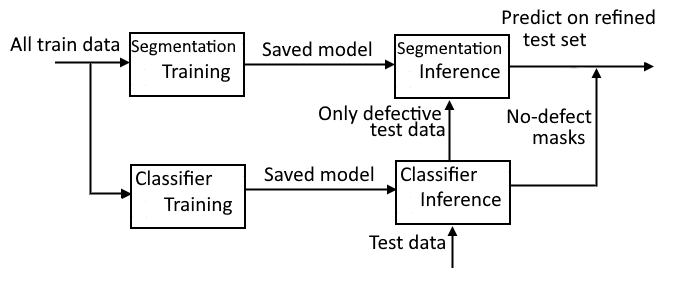
\includegraphics[scale=0.48]{Img_SecondApproach}
   \end{figure}


   \subsection{Multiclass Semantic Segmentation}
   The semantic segmentation task is performed by a U-Net based model. In my experiments, I have tried three different U-Net encoders: ResNet34, ResNet50 and EfficientNet-B3. In the following, I will refer to the EfficientNet-B3 model only since it has given the best result (Table \ref{table:res_encoders}.).
   The main advantage of using custom encoders is that it is possible to apply transfer-learning from pretrained weights, allowing to transfer previous knowledge to the network. \\
   The encoder part follows the EfficientNet-B3 architecture \cite{efficientnet}. The decoder part, instead, is a classical U-Net expansion path, where each upsampling layer is concatenated with the corresponding downsampling one in the contracting part, followed by a block of Convolution, Batch-Normalization and ReLu layer. \\
   The decision about the right activation layer at the end of the network was a great challenge for quite a long time: even if Softmax is the straightforward choice for multiclass segmentation by definition, this means that I have to treat 'no Defect' pixels as a separate class altogether. In my opinion, this decision will stress even more the imbalanced data issue, since for each pixel it is necessary to decide the right class, where, as I presented in the dataset analysis, it is clear that almost the entire amount of pixels belongs to the non-defective group. The usage of the Sigmoid activation function, instead, brings the network to perform four \textit{one vs all} independent decisions, whether that pixel belongs to the corresponding class or not. The experiment results seems inline with the above intuition (Table \ref{table:res_encoders})

   \subsection{Binary Classification}
   The classification task is delegated to a standard binary classifier. In my experiments, I have tried two different models: ResNet34 and ResNet50. In the following, I will refer to ResNet50 only, because it has performed the best result.
   The structure of the classifier follows the classical ResNet50 architecture \cite{resnet}, then the last part of Fully Connected layers is removed and replaced by a Global Averaging Pooling layer attached with a sigmoid activation over the single binary output.


%%%%%%%%% EXPERIMENTS
%------------------------------------------------------------------------
\section{Experiments}
   The entire pipeline is trained separately, so for a legibility purpose, I will divide the two experiments and then provide the final results using the Dice coefficient \eqref{eq:dice_loss}.
   \begin{equation}\label{eq:dice_loss}
      L_{dice} = \frac{2 * y_{pred} * y_{true}}{y_{pred} + y_{true}}
   \end{equation}

   \subsection{Dataset analysis}
   The dataset is obtained from the corresponding Kaggle competition \cite{Severstal}. It is composed of 12568 greyscale images of size 1600x256x3 and their corresponding defective masks.
   The dataset exhibits a fairly even distribution between defective (56\%) and non-defective images (44\%), but among the defective ones we can notice a strong imbalance between defect classes (Figure \ref{fig:classImbalance}). This distribution can lead to recognize only one type of defect (the third one), since it represents the largest part of the defective images.
   \begin{figure}[h]
      \centering
      \caption{Defect class distribution} \label{fig:classImbalance}
      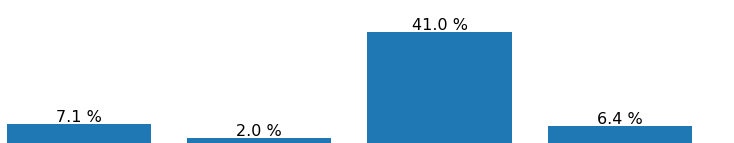
\includegraphics[scale=0.45]{Img_ClassImbalance}
   \end{figure}

   \subsection{Segmentation}
      \paragraph{Data preparation}
         The first operation applied is to crop the images due to the large dimensions of the input data and the corresponding limited amount of memory. Thanks to the idea behind Fully Convolutional Neural Network, it is possible to train and predict on different image dimensions with good output resolution \cite{FCNN}.
         In order to apply a first level of data augmentation, the crop size varies on different epochs, also completely dark crops are prevented since they do not bring any useful information.
         In order to face the imbalanced dataset issue, the batch is composed of all images' classes in equal proportion (included non-defective class).

      \paragraph{Training parameters}
         \begin{itemize}
            \item Data augmentation is applied with both random spatial transformations (flip, rotation and shifting) and color augmentation (brightness and contrast).
            \item The crop size used are (5, 256, 384) and (5, 256, 512) that will interchange on epochs, where the first number in the tuple identifies the batch size.
            \item The loss function varies during the training: the first 70 epochs were trained using a balanced combination of two loss functions, Binary Cross Entropy and Dice \eqref{eq:dice_loss}, that provides a tradeoff between accuracy and precision \eqref{eq:loss_bce_dice}. Finally, the model is fine tuned for other 40 epochs using Tversky loss \eqref{eq:loss_tversky}, \cite{tversky} with \textalpha=0.3, to reduce the false positive rate. In the class of softmax activation function, the loss used is Categorical Cross Entropy working on channel axis.
            \begin{equation}\label{eq:loss_bce_dice}
               L_{bce\_dice} = L_{dice} + L_{bce}
            \end{equation}
            \begin{equation}\label{eq:loss_tversky}
               L_{Tversky} = \frac{TP}{TP + \alpha*FN + (1-\alpha)*FP}
            \end{equation}
            \item The network is optimized using Adam, with an initial learning rate of $ 10^{-3} $ that is reduced with a constant factor of 0.5 every time it reaches a plateau long three epochs.
         \end{itemize}

      \paragraph{Experimental results and observations}
         The followig results refer to tests on the segmentation model only (Table \ref{table:res_encoders}).
         \begin{table}[h]
            \centering
            \begin{tabular}{||c c c||} 
            \hline
            Encoder model & Activation function & Dice metric\\ [0.4ex] 
            \hline\hline
            ResNet34 & Sigmoid & 0.469 \\ 
            \hline
            ResNet50 & Sigmoid & 0.602 \\
            \hline
            \textbf{EfficientNet-B3} & \textbf{Sigmoid} & \textbf{0.607} \\
            \hline
            EfficientNet-B3 & Softmax & 0.509 \\
            \hline
            \end{tabular}
            \caption{Results on different encoders and activation functions}
            \label{table:res_encoders}
         \end{table}

         As I mentioned before, U-Net provides a very accurate identification of defects, but hardly distinguishes real defects from the false ones, that usually are identified as small scarfs in the steel (Figure \ref{fig:result1}). 
         \begin{figure}[h]
            \centering
            \caption{Real (purple) vs False (blue) defects} \label{fig:result1}
            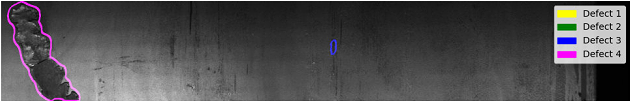
\includegraphics[scale=0.5]{Img_Result1.png}
         \end{figure}
         \\This would not be a big issue if the challenges' metrics does not penalize so much false defects on non-defective images, even if they are a small proportion of the entire image(Figure \ref{fig:result2}).  
         \begin{figure}[h]
            \centering
            \caption{False defects on good image} \label{fig:result2}
            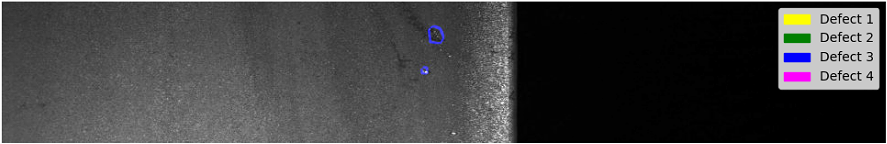
\includegraphics[scale=0.355]{Img_Result2.png}
         \end{figure}
   
   \subsection{Classification}
      \paragraph{Data preparation} 
         For the classification, no data preprocessing has been applied.
                 
      \paragraph{Training parameters}
      \begin{itemize}
         \item Data augmentation is applied with both random spatial transformations (flip, rotation and shifting) and color augmentation (brightness and contrast).
         \item The images are fed on their original size of (4, 256, 1600), where the first number in the tuple identifies the batch size.
         \item The loss function is Binary Cross Entropy. 
         \item The network is optimized using Adam, with an initial learning rate of $ 10^{-3} $ that is reduced with a constant factor of 0.5 every time it reaches a plateau long three epochs.
      \end{itemize}

      \paragraph{Experimental results and observations}
         The followig results refer to tests on the classification model only.
         \begin{table}[!htb]
            \begin{minipage}{.5\linewidth}
               \begin{tabular}{cc|cc}
               \multicolumn{1}{c}{} &\multicolumn{1}{c}{} &\multicolumn{2}{c}{Predicted} \\ 
               \multicolumn{1}{c}{} & 
               \multicolumn{1}{c|}{} & 
               \multicolumn{1}{c}{True} & 
               \multicolumn{1}{c}{False} \\ \hline
               \multirow[c]{2}{*}{\rotatebox[origin=tr]{90}{Real}}
               & True  & 662 & 54   \\[1.5ex]
               & False  & 373   & 711 \\ \hline
               \end{tabular}
               \caption{Resnet34}
               \label{table:resnet34_cm}
            \end{minipage}%
            \begin{minipage}{.5\linewidth}
               \begin{tabular}{@{}cc|cc@{}}
               \multicolumn{1}{c}{} &\multicolumn{1}{c}{} &\multicolumn{2}{c}{Predicted} \\ 
               \multicolumn{1}{c}{} & 
               \multicolumn{1}{c|}{} & 
               \multicolumn{1}{c}{True} & 
               \multicolumn{1}{c}{False} \\ 
               \cline{2-4}
               \multirow[c]{2}{*}{\rotatebox[origin=tr]{90}{Real}}
               & True  & \textbf{695} & \textbf{21}   \\[1.5ex]
               & False  & \textbf{365}   & \textbf{719} \\ 
               \cline{2-4}
               \end{tabular}
               \caption{Resnet50}
               \label{table:resnet50_cm}
            \end{minipage} 
         \end{table} 
         As it can be seen from the confusion matrix above, the classification helps to identify most of the non-defective images and avoid the segmentation step, that in some cases can create only problems. The most important thing here is to keep the False Negative rate as small as possible, in order not to skip the segmentation of defective images.
            
   \subsection{Complete pipeline}
      The training procedure of the entire pipeline is simply composed of the two procedures stated above.
      The following refers to the results coming from the two approaches, using EfficientNet-B3 as encoder model of the U-Net in the segmentation phase, and ResNet50 as binary classifier. 
      \begin{table}[h]
         \centering
         \begin{tabular}{||c c||} 
         \hline
         Approach & Dice coefficient\\ [0.5ex] 
         \hline\hline
         Segmentation only & 0.607 \\ 
         \hline
         \textbf{Complete pipeline} & \textbf{0.729} \\
         \hline
         \end{tabular}
         \caption{Results on different approaches}
         \label{table:res_finals}
      \end{table}


%%%%%%%%% CONCLUSION
%-----------------------------------------------------------------------
\section{Conclusion} 
   This project leverages the semantic segmentation and classification techniques to solve the steel defect detection problem. From the experiments, it arises that the combination of these two techniques works particularly well as a tradeoff between accuracy and precision, in this particular field.\\
   Possible future improvements could be:
   \begin{itemize}
      \item Try ensemble learning, in order to exploit the capability of different encoder models.
      \item Fight the imbalanced dataset issue using a custom loss that takes in consideration the defect class distribution.
   \end{itemize}
   It is possible to find all the code and experiments at the following github repository: \url{https://github.com/AndreaBiondaPolimi/Severstal_Segmentation/tree/master}


   

{\small
\bibliographystyle{ieee}
\bibliography{egbib}
}

\end{document}
